
\documentclass[11pt, a4paper]{article}
%\usepackage{proj1}
\usepackage{natbib}
\usepackage{fancyhdr}  
\usepackage{subcaption}
\usepackage{caption}
\usepackage{graphicx}
\usepackage{numprint}
\usepackage{multirow}
\linespread{1.25} 
\setlength{\parindent}{0cm}
\graphicspath{{Images/}}
\usepackage{hyperref}
\usepackage{amsmath}
\usepackage{amsfonts}
\usepackage{amssymb}
\usepackage{amsthm}
\usepackage{mathtools}
\usepackage{commath}
\usepackage{bbm}

%\usepackage[sc,osf]{mathpazo}
\usepackage{subcaption}
\usepackage[a4paper, top=1in, left=1.0in, right=1.0in, bottom=1in, includehead, includefoot]{geometry} %Usually have top as 1in

\usepackage{listings}
\usepackage{color} %red, green, blue, yellow, cyan, magenta, black, white
\definecolor{mygreen}{RGB}{28,172,0} % color values Red, Green, Blue
\definecolor{mylilas}{RGB}{170,55,241}


\hypersetup{colorlinks,linkcolor={black},citecolor={blue},urlcolor={black}}
\usepackage{color}
\urlstyle{same}


\theoremstyle{definition}
\newtheorem{definition}{Definition}[section]

\newcommand{\adja}{q_a}
\newcommand{\adjb}{q_b}
\newcommand{\adjaB}{q_{a,\partial \Omega}}
\newcommand{\adjbB}{q_{b,\partial \Omega}}
\newcommand{\adjB}{q_{\partial \Omega}}
\newcommand{\Adja}{\mathbf{p}}
\newcommand{\Adjb}{q}
\newcommand{\adj}{q}
\newcommand{\Adjc}{{q}_{\partial \Omega}}
\newcommand{\ra}{\rho_a}
\newcommand{\rb}{\rho_b}
\newcommand{\w}{\mathbf{w}}
\newcommand{\x}{\mathbf{x}}
\newcommand{\f}{\mathbf{f}}
\newcommand{\ve}{\mathbf{v}}
\newcommand{\n}{\mathbf{n}}
\newcommand{\h}{\mathbf{h}}
\newcommand{\K}{\mathbf{K}}
\newcommand{\hr}{\widehat \rho}
\newcommand{\jf}{\mathbf j}

\DeclareMathOperator{\sgn}{sgn}
\DeclareMathOperator{\Grad}{Grad}
\DeclareMathOperator{\Div}{Div}
\DeclareMathOperator{\Lap}{Lap}
%	\begin{figure}[h]
%		\centering
%		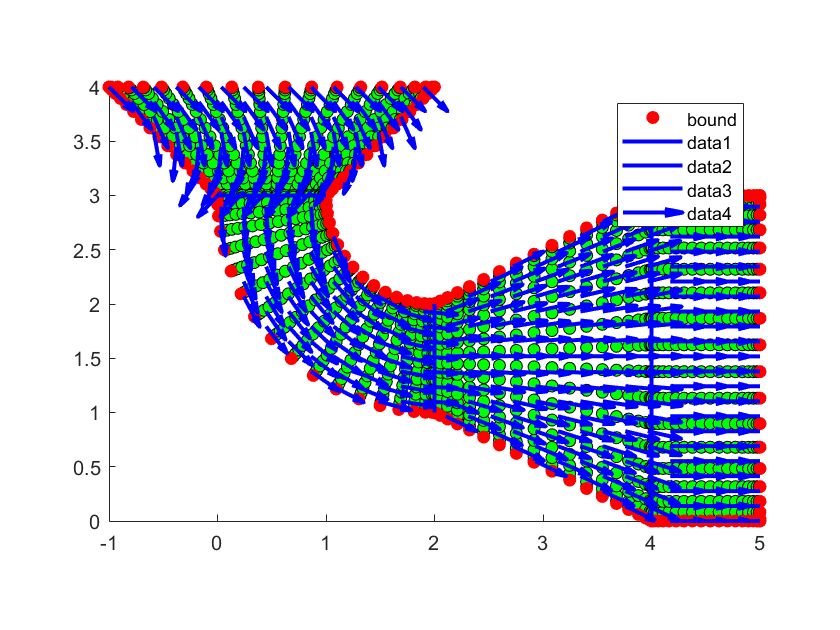
\includegraphics[scale=0.35]{F1.png}
%		\caption{Forward $\rho$ for $a = 0.01$} 
%		\label{F1}
%	\end{figure}

\begin{document}
++ maybe Dirichlet non-zero (i.e. positive) and scale to 1? +++ 	
	\section{Green's theorem stuff}
	We wrote the terms in * and ** into vector form as (*, **), but it should have been * + **. I think it has to be a sum, since the term we start out with in the cost functional is the scalar quantity
	\begin{align*}
		\frac{1}{2} \int_\Omega \nabla \times \w ^2 d\x &= \frac{1}{2} \int_\Omega \left(\frac{\partial w_2}{\partial x_1} - \frac{\partial w_1}{\partial x_2}\right)^2 d\x\\
		&= \int_\Omega \frac{1}{2} \frac{\partial w_2}{\partial x_1}\frac{\partial w_2}{\partial x_1} - \frac{\partial w_2}{\partial x_1}\frac{\partial w_1}{\partial x_2} + \frac{1}{2}\frac{\partial w_1}{\partial x_2}\frac{\partial w_2}{\partial x_1} d\x.
	\end{align*}
	We take the derivative with respect to $h_1$, $h_2$
	\begin{align*}
		&\int_\Omega  \frac{\partial h_2}{\partial x_1}\frac{\partial w_2}{\partial x_1} - \frac{\partial h_2}{\partial x_1}\frac{\partial w_1}{\partial x_2} - \frac{\partial w_2}{\partial x_1}\frac{\partial h_1}{\partial x_2}+ \frac{\partial h_1}{\partial x_2}\frac{\partial w_1}{\partial x_2} d\x \\
		=&\int_\Omega \frac{\partial h_2}{\partial x_1} \left(\frac{\partial w_2}{\partial x_1} - \frac{\partial w_1}{\partial x_2} \right) + \frac{\partial h_1}{\partial x_2}\left(\frac{\partial w_1}{\partial x_2} - \frac{\partial w_2}{\partial x_1} \right) d\x\\
		=& \int_\Omega \frac{\partial}{\partial x_1}\left(h_2\frac{\partial w_2}{\partial x_1} - h_2\frac{\partial w_1}{\partial x_2} \right) - \left(h_2\frac{\partial^2 w_2}{\partial x_1^2} - h_2\frac{\partial^2 w_1}{\partial x_1 x_2} \right)\\
		& + \frac{\partial}{\partial x_2}\left(h_1\frac{\partial w_1}{\partial x_2} - h_1\frac{\partial w_2}{\partial x_1} \right) - \left(h_1\frac{\partial^2 w_1}{\partial x_2^2} - h_1\frac{\partial^2 w_2}{\partial x_1 x_2} \right) d\x.
	\end{align*}
	Applying Green's theorem, we get
	\begin{align*}
		&\int_{\partial \Omega}\left(h_2\frac{\partial w_2}{\partial x_1} - h_2\frac{\partial w_1}{\partial x_2} \right) dx_1 + \left(h_1\frac{\partial w_1}{\partial x_2} - h_1\frac{\partial w_2}{\partial x_1} \right)dx_2\\
		&- \int_\Omega \left(h_2\frac{\partial^2 w_2}{\partial x_1^2} - h_2\frac{\partial^2 w_1}{\partial x_1 x_2} \right) + \left(h_1\frac{\partial^2 w_1}{\partial x_2^2} - h_1\frac{\partial^2 w_2}{\partial x_1 x_2} \right)  d\x.
	\end{align*}
	Rewriting the boundary terms we get
	\begin{align*}
		&\int_{\partial \Omega}\nabla \times \w h_2 dx_1 - \nabla \times \w h_1 dx_2\\
		&- \int_\Omega \left(h_2\frac{\partial^2 w_2}{\partial x_1^2} - h_2\frac{\partial^2 w_1}{\partial x_1 x_2} \right) + \left(h_1\frac{\partial^2 w_1}{\partial x_2^2} - h_1\frac{\partial^2 w_2}{\partial x_1 x_2} \right)  d\x.
	\end{align*}
	Green's Theorem can be written as
	\begin{align*}
		\int_{\partial \Omega} Ldx + M dy = \int_{\partial \Omega} \left(M, - L\right) \cdot \left(dy, - dx\right) = \int_{\partial \Omega} \left(M, - L\right) \cdot \n ds,
	\end{align*}
	where $ds = \sqrt{dx^2 + dy^2}$ and $\n$ chosen such that it is normalized and perpendicular to $(dx, dy)$.
	Therefore, we have
	\begin{align*}
		\int_{\partial \Omega}\nabla \times \w h_2 dx_1 - \nabla \times \w h_1 dx_2 &= \int_{\partial \Omega}\nabla \times \w \left(-h_1, - h_2\right)\cdot (dx_2, - dx_1) \\
		&= \int_{\partial \Omega}\nabla \times \w \left(-h_1, - h_2\right) \cdot \left(\frac{dx_2}{ds}, - \frac{dx_1}{ds}\right) ds,
	\end{align*}
	Consider the boundary term from my derivation	
	\begin{align}
		& \int_{\partial \Omega} \left(\nabla \times \w\right) \h_\bot \cdot \n d s\notag\\
		=&  \int_{\partial \Omega} \left(\nabla \times \w\right) \left(h_2, - h_1\right) \cdot (n_1, n_2) d s \label{eq1}.
	\end{align}
	These two formulations agree if $n_1 = \frac{dx_1}{ds}$ and $n_2 = \frac{dx_2}{ds}$. However, this doesn't quite make sense to me, since these are not normal to $dx_1$ and $dx_2$.
	\subsection{Quick reminder on what I've done }
	We know that
	\begin{align*}
		\nabla \times \w = \nabla \cdot  \w_\bot,
	\end{align*}
	where $\w_\bot = (w_2 , -w_1)$, the result of a rotation of $\w$ by $\pi/2$.
	The Lagrangian included a term of the form
	\begin{align*}
		\mathcal L (\rho, \w ,q) =& ...  \frac{\eta}{2}\int_0^T \int_\Omega \left(\nabla \cdot  \w_\bot\right)^2 d\x dt ...
	\end{align*}
	For the adjoint equation, we find the usual results.
	We take the derivative with respect to $\w$
	\begin{align*}
		\mathcal L_\w(\rho, \w, q)\h &= \int_0^T \int_\Omega ... + \eta \left(\nabla \cdot  \h_\bot\right) \left(\nabla \cdot  \w_\bot\right)d\x dt.
	\end{align*}
	Then we integrate by parts (or divergence theorem) to get
	\begin{align*}
		\mathcal L_\w(\rho, \w, q)\h &= \int_0^T \int_\Omega.... - \eta \nabla\left(\nabla \cdot  \w_\bot\right)  \cdot \h_\bot d\x dt + \int_0^T \int_{\partial \Omega} \eta \left(\nabla \cdot  \w_\bot\right) \h_\bot \cdot \n d \x dt.
	\end{align*}
	\section{Paper Examples}
	\section*{Source Control Neumann}
	We choose 
	\begin{align*}
		\rho_0 &= 0.25\\
		V_{ext} &= 1.5\sin(\pi x_2/5)\cos(\pi x_1/5 + \pi/5)\\
		\hr &= 0.25(1 - t) + t(0.25\sin(\pi(x_1 - 2)/2)\sin(\pi(x_2 - 2)/2) + 0.25)
	\end{align*}
	We choose the domain $[-1,1]^2$ with a time horizon $(0,1)$. We have $N = 20$, $n = 11$. 
	With $\beta = 10^{-3}$ we solve this problem in $333$ seconds. When $\kappa = 1$, the cost functional is $J = 0.015$, $J_1 = 0.021$ and $J_2 = 0.9946$. (We compare this against the result with $\beta = 10^3$, where we get $J = 0.0153$. For $\beta = 10^{-5}$ we get $J = 8.5366 \times 10^{-4}$, see Figure \ref{F1c}.)
	Figure \ref{F1} displays the results, Figure \ref{F1a} shows the external potential acting on the particles.
	\begin{figure}[h]
		\centering
		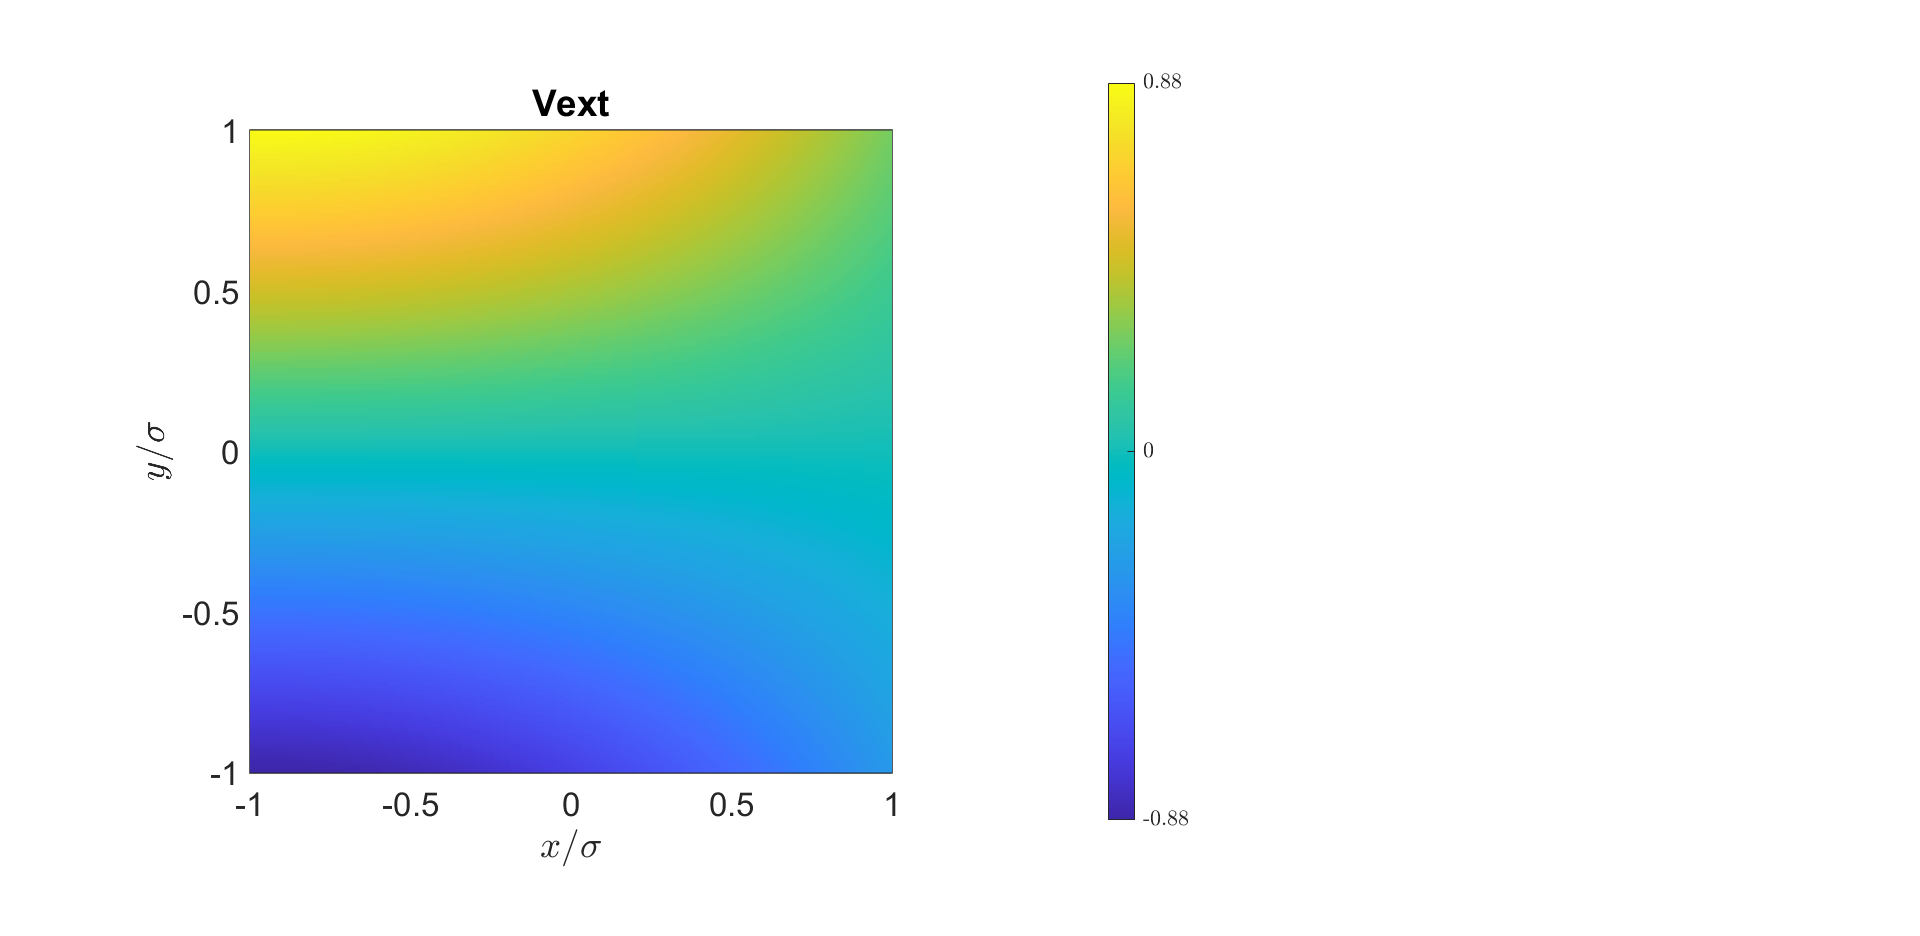
\includegraphics[scale=0.35]{Vext.png}
		\caption{$V_{ext}$ corresponding to results in Figure \ref{F1}.} 
		\label{F1a}
	\end{figure}
	\begin{figure}[h]
		\centering
		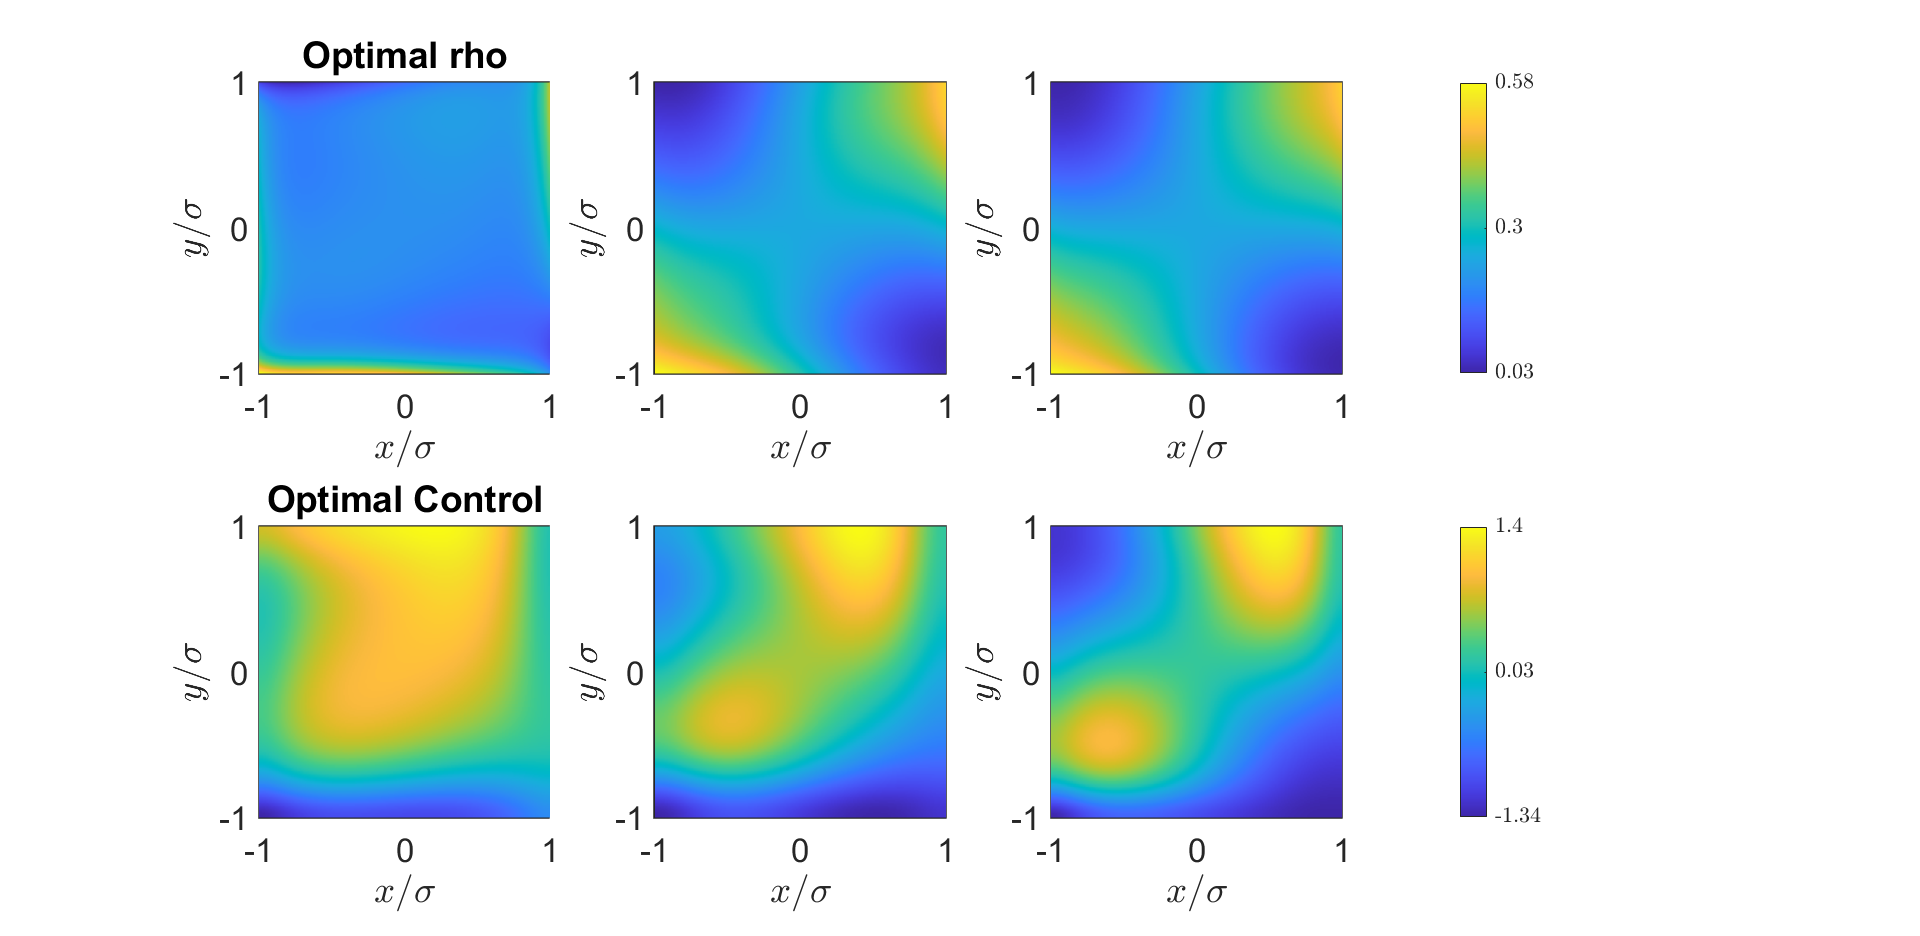
\includegraphics[scale=0.35]{SCEx1k1.png}
		\caption{Optimal $\rho$ and cost $w$, $\kappa = 1$, $\beta = 10^{-3}$} 
		\label{F1}
	\end{figure}
	
	For $\kappa = -1$ we get $J = 0.013$, $J_1 = 0.017$ and $J_2 = 0.8846$. The result can be seen in Figure \ref{F1b}.(We compare this against the result with $\beta = 10^3$, where we get $J = 0.0171$. For $\beta = 10^{-5}$ we get $J = 8.0800 \times 10^{-4}$, see Figure \ref{F1d}.)
	We can see that the control behaviour for $\kappa = -1$ is very different to the one for $\kappa = 1$, since the repulsion supports the drive towards $\hr$, while the attraction counteracts it. For both cases we can observe that the control works harder in regions with steep external potential.
	\begin{figure}[h]
		\centering
		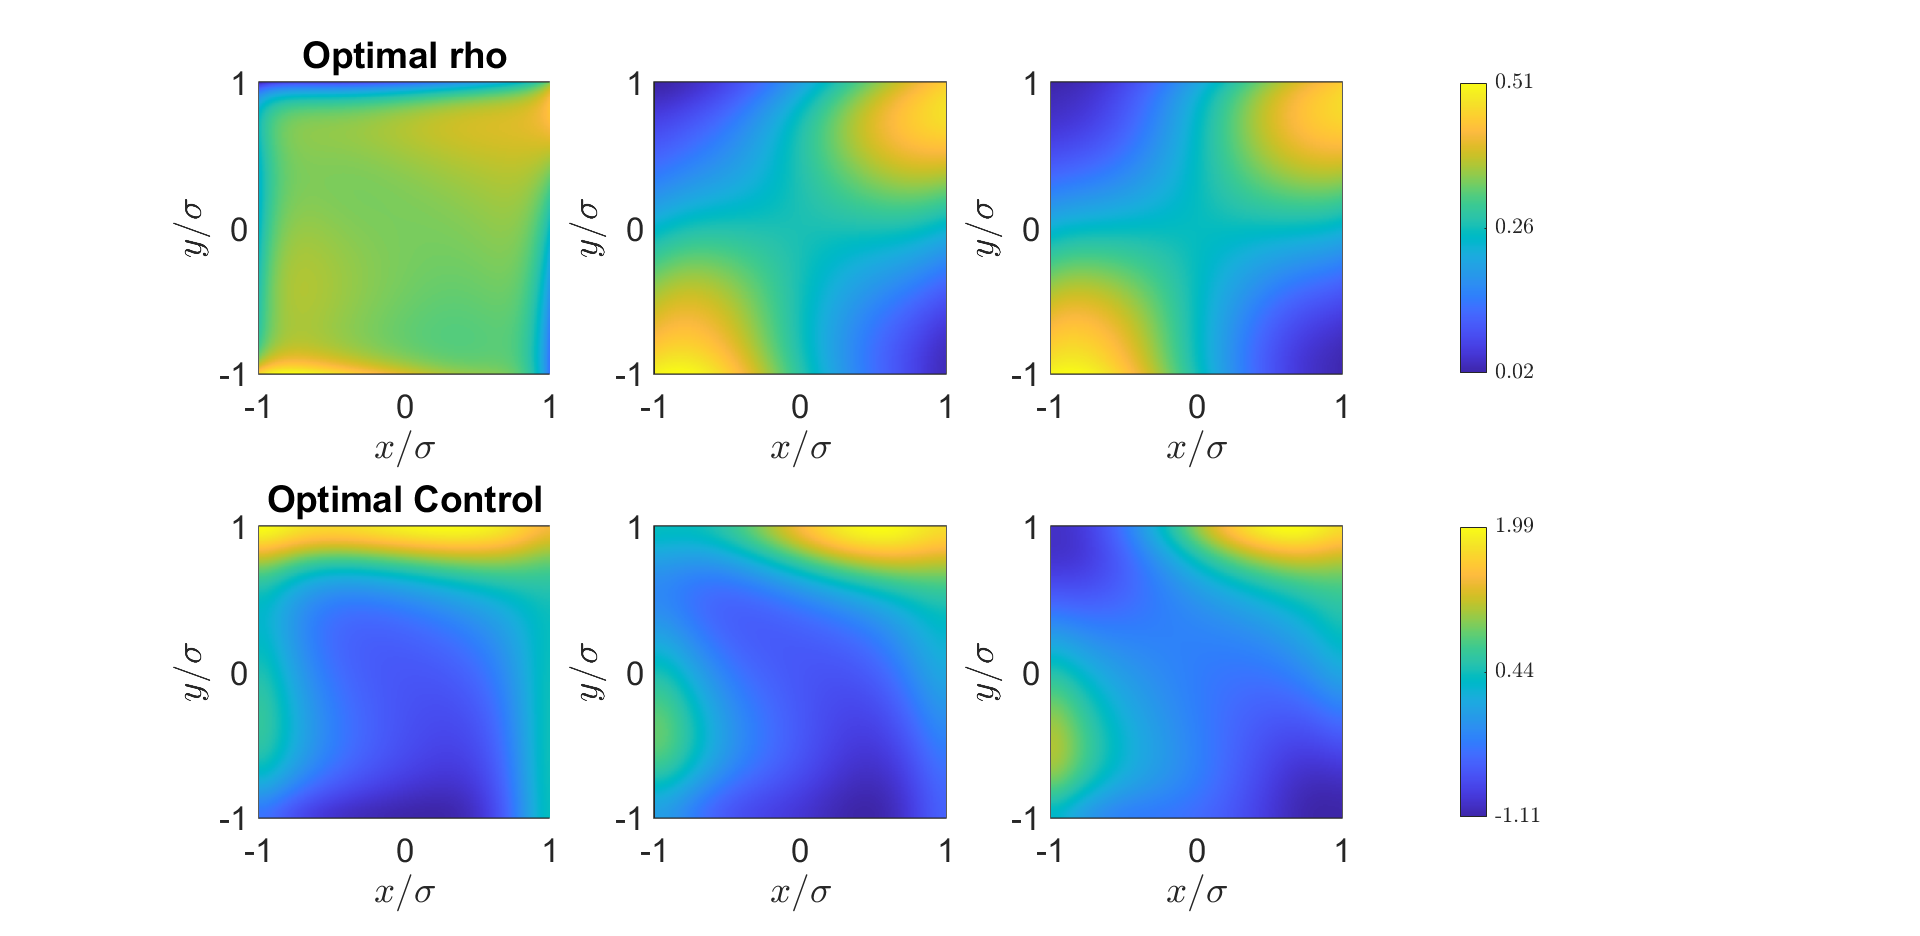
\includegraphics[scale=0.35]{SCEx1kn1.png}
		\caption{Optimal $\rho$ and cost $w$, $\kappa = - 1$, $\beta = 10^{-3}$.} 
		\label{F1b}
	\end{figure}

	\begin{figure}[h]
		\centering
		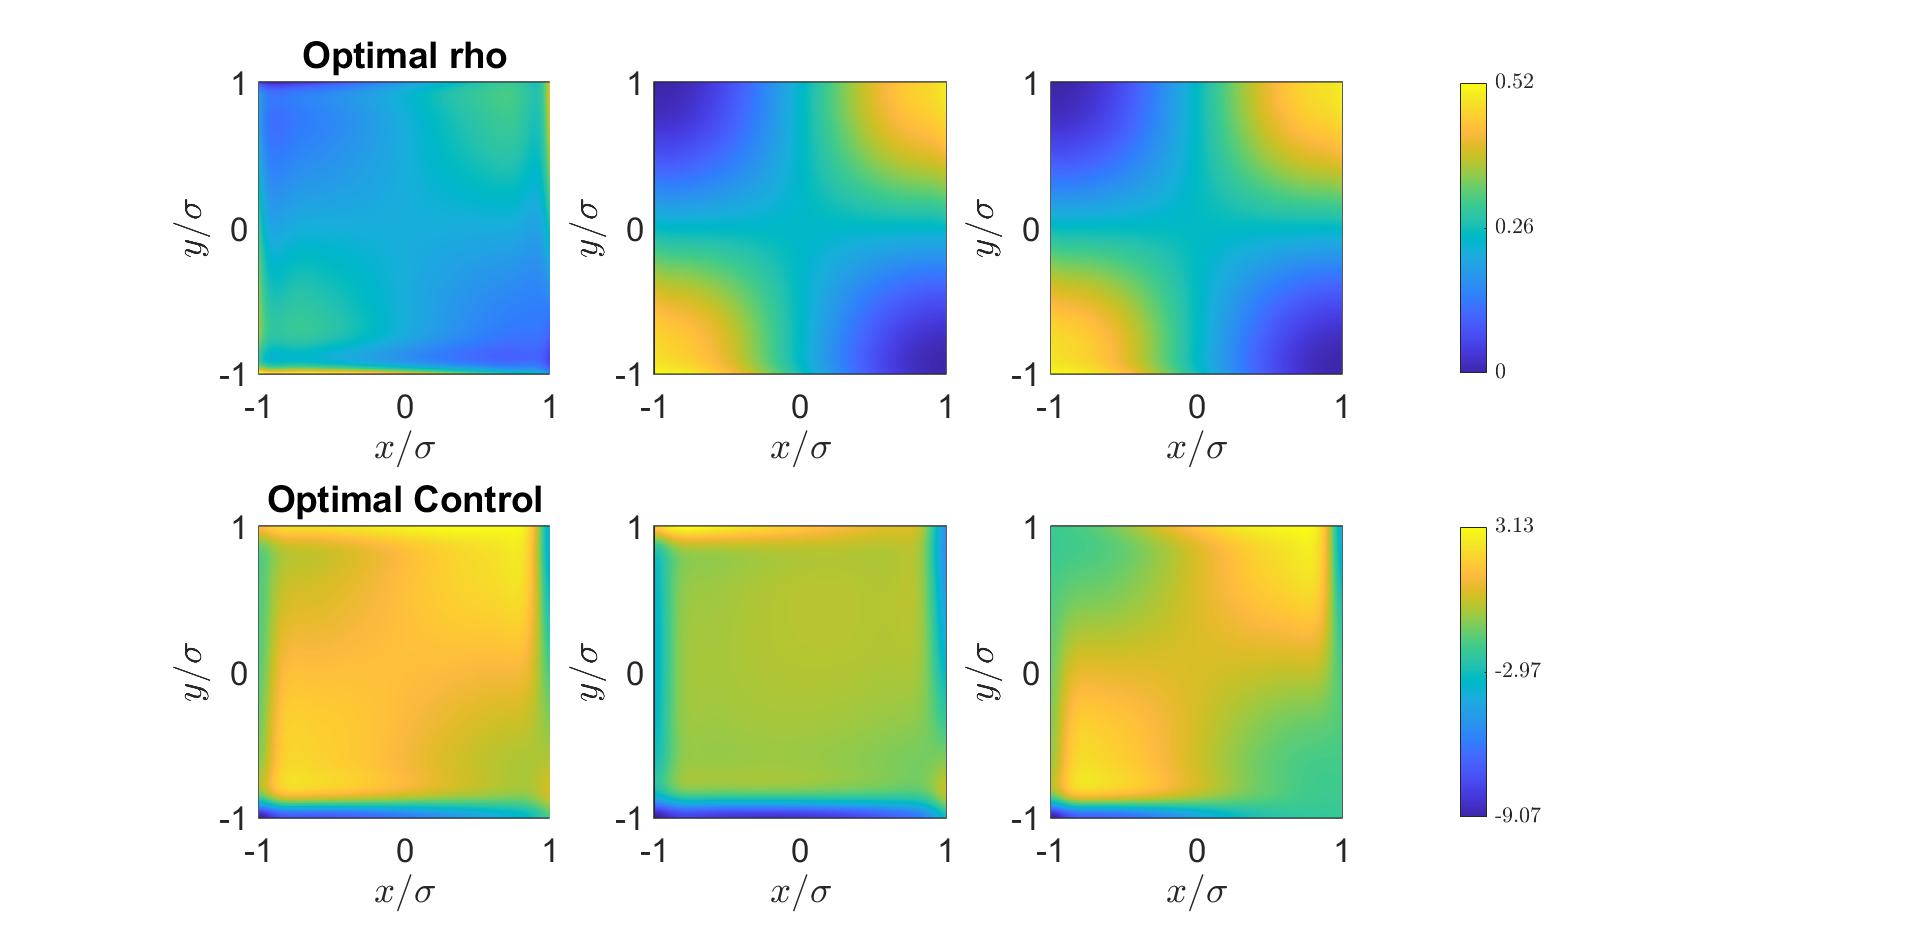
\includegraphics[scale=0.35]{SCEx1k1b5.png}
		\caption{Optimal $\rho$ and cost $w$, $\kappa = 1$, $\beta = 10^{-5}$.} 
		\label{F1c}
	\end{figure}
	\begin{figure}[h]
		\centering
		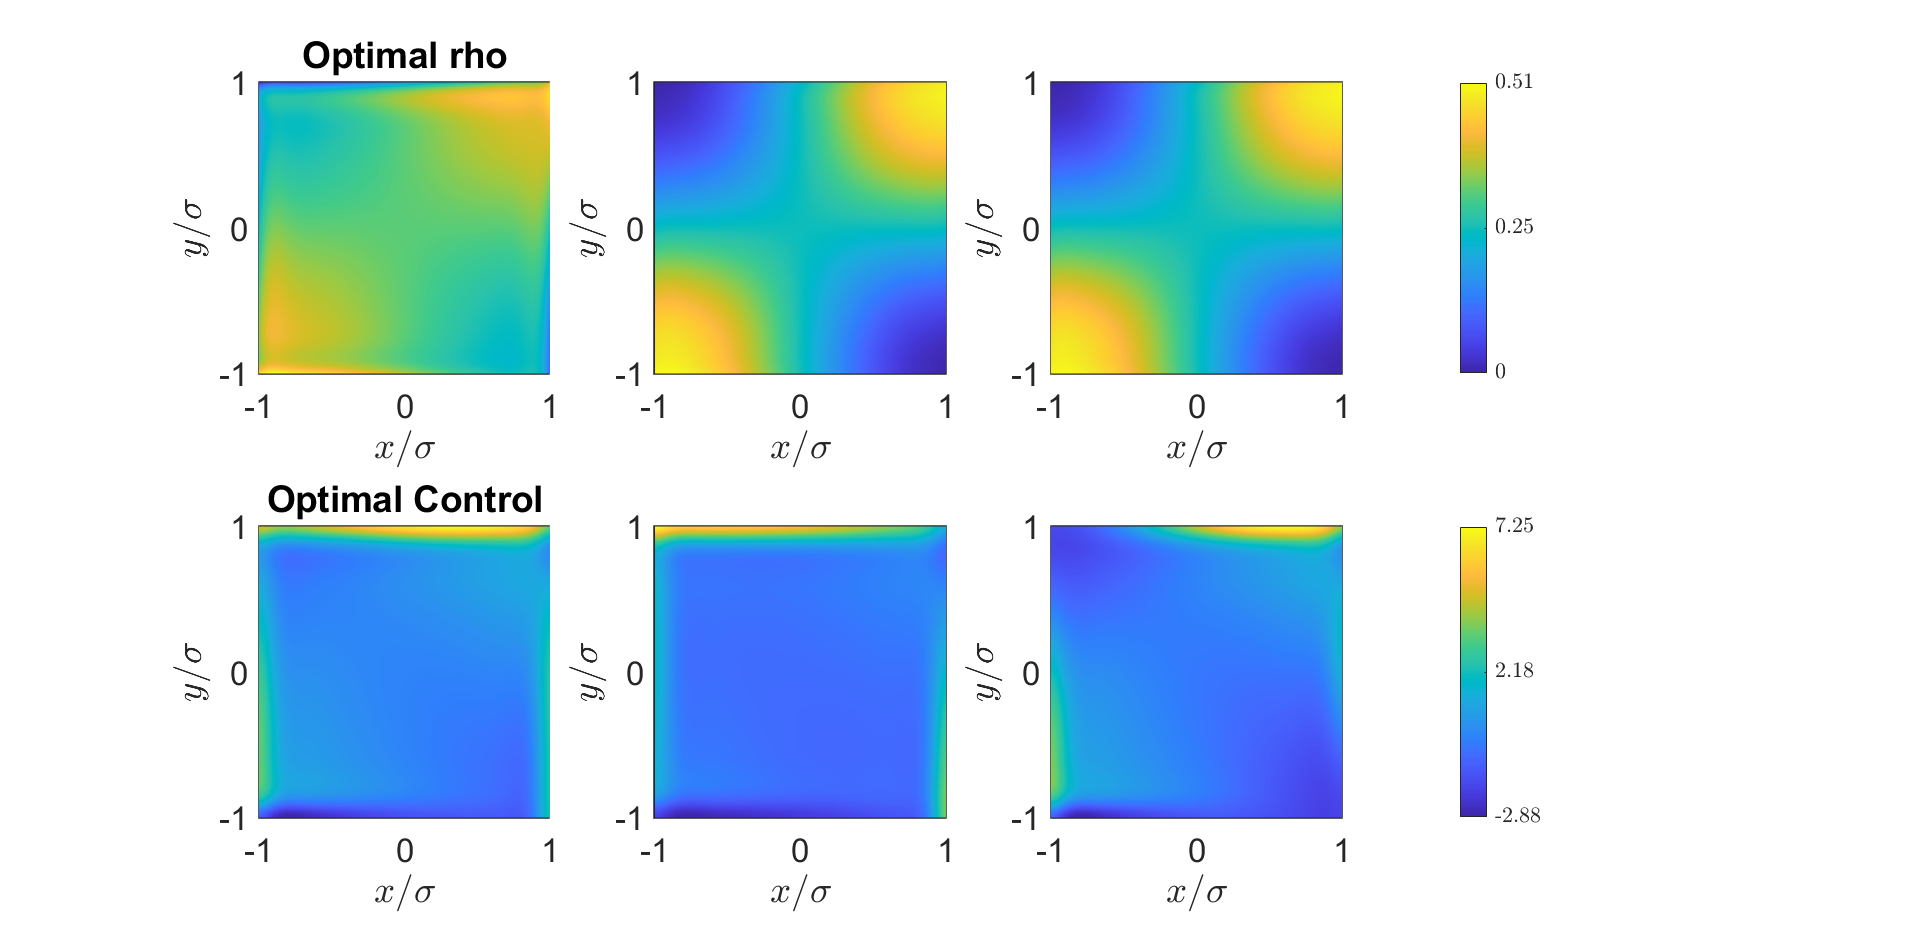
\includegraphics[scale=0.35]{SCEx1kn1b5.png}
		\caption{Optimal $\rho$ and cost $w$, $\kappa = - 1$, $\beta = 10^{-5}$.} 
		\label{F1d}
	\end{figure}
	\section*{Source Control Dirichlet}
		We choose 
	\begin{align*}
		\rho_0 &= 0.25\cos(\pi x_1/2)\cos(\pi x_2/2)\\
		V_{ext} &=  (1-t)(-\cos(\pi x_1/2)\sin(\pi x_2/2) + 1)\\
		\hr &= 0.25\cos(\pi x_1/2)\cos(\pi x_2/2)(1 - t) - t\sin(\pi x_1)\sin(\pi x_2/2 - \pi/2)
	\end{align*}
	We choose the domain $[-1,1]^2$ with a time horizon $(0,1)$. We have $N = 20$, $n = 11$. 
	For $\beta = 10^{-3}$, $\kappa =1$ we get $J = 0.0268$, $J_1 = 0.0096$ and $J_2 = 43.9790$. (vs $\beta = 10^3$, where $J = 0.1709$.)
	For $\beta = 10^{-3}$, $\kappa =1$ we get $J = 0.0257$, $J_1 = 0.0089$ and $J_2 = 42.4812$. (vs $\beta = 10^3$, where $J = 0.1707$.) Both example take around $60$ to $80$ seconds to solve.
	\begin{figure}[h]
		\centering
		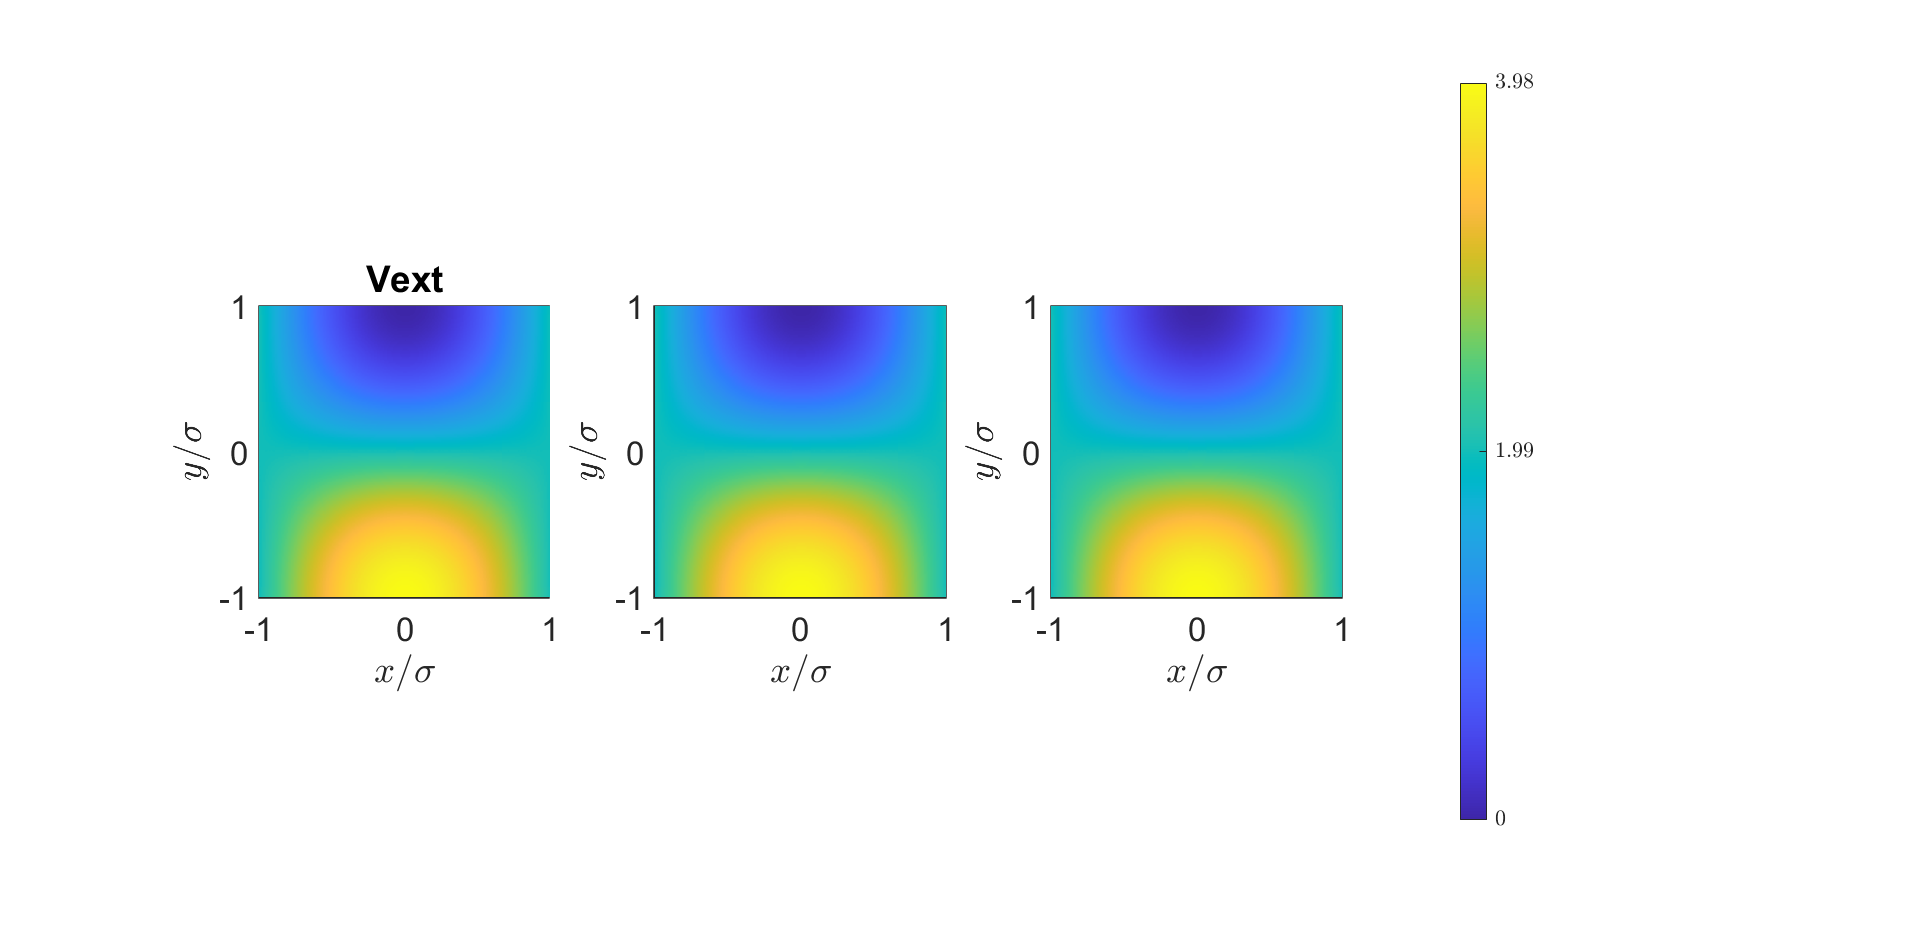
\includegraphics[scale=0.35]{VextEx2.png}
		\caption{$V_{ext}$ corresponding to results in Figure \ref{F2}.} 
		\label{F2a}
	\end{figure}
	\begin{figure}[h]
		\centering
		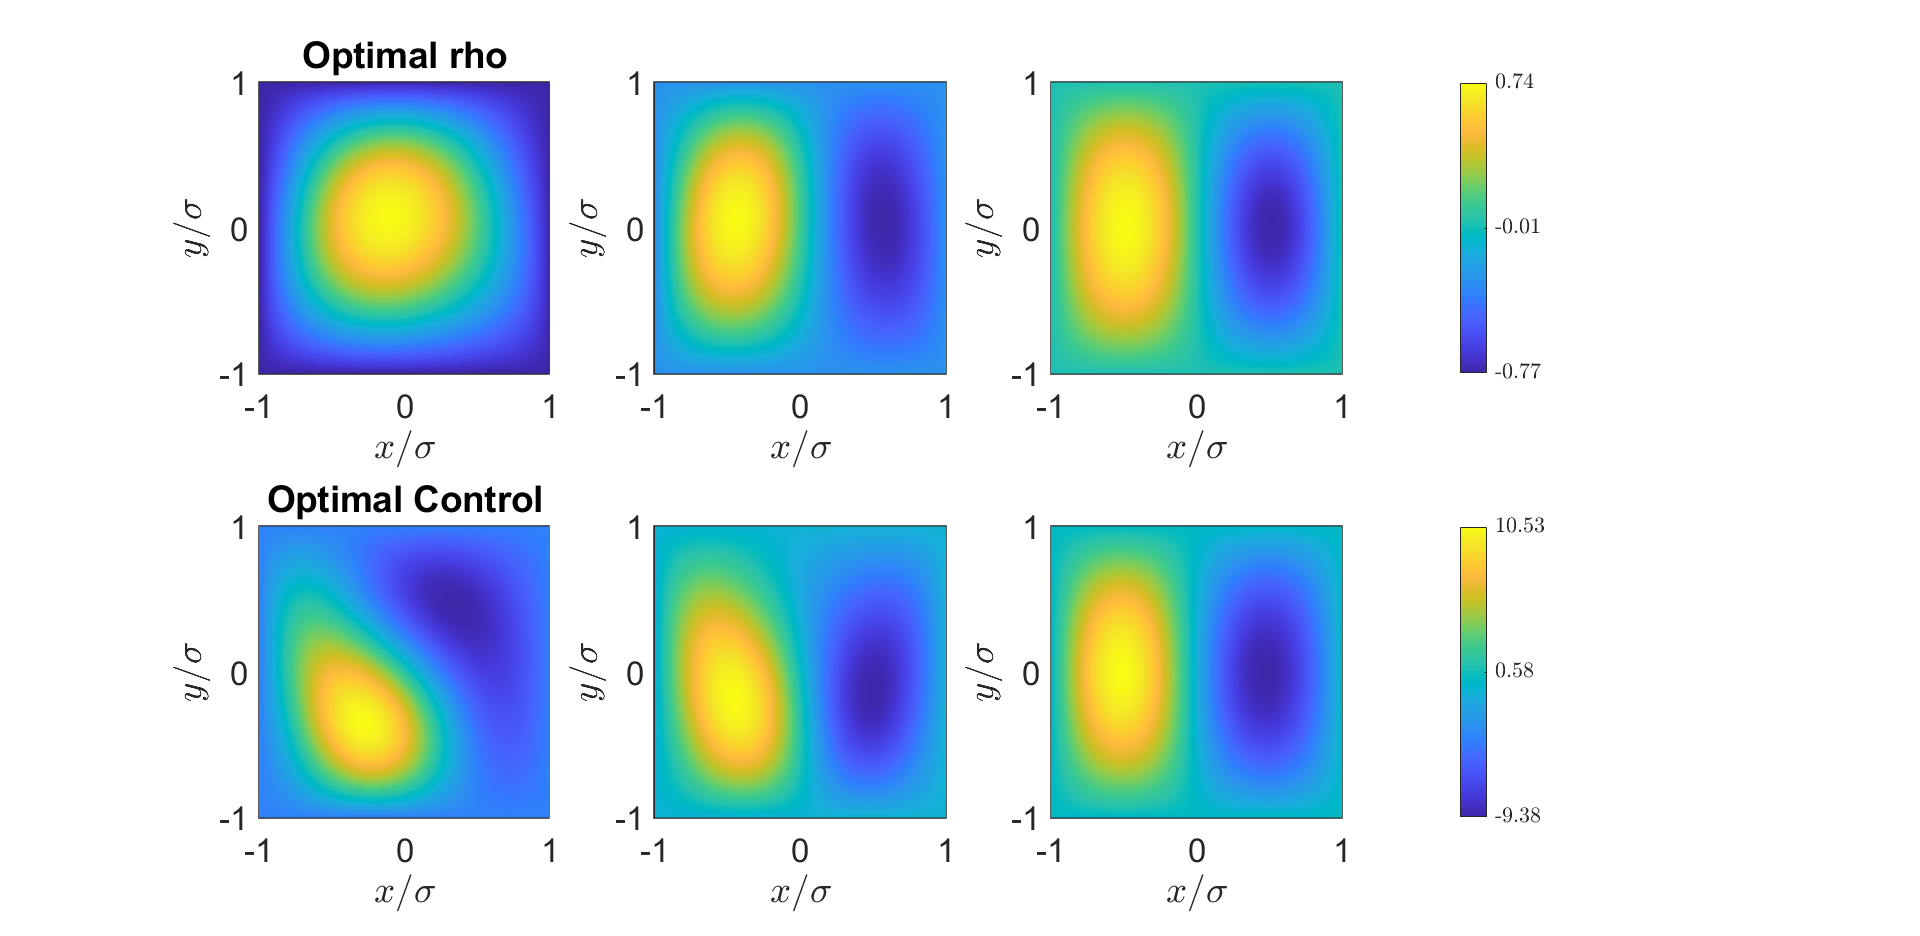
\includegraphics[scale=0.35]{SCEx2k1V.png}
		\caption{Optimal $\rho$ and cost $w$, $\kappa = 1$.} 
		\label{F2}
	\end{figure}
	\begin{figure}[h]
		\centering
		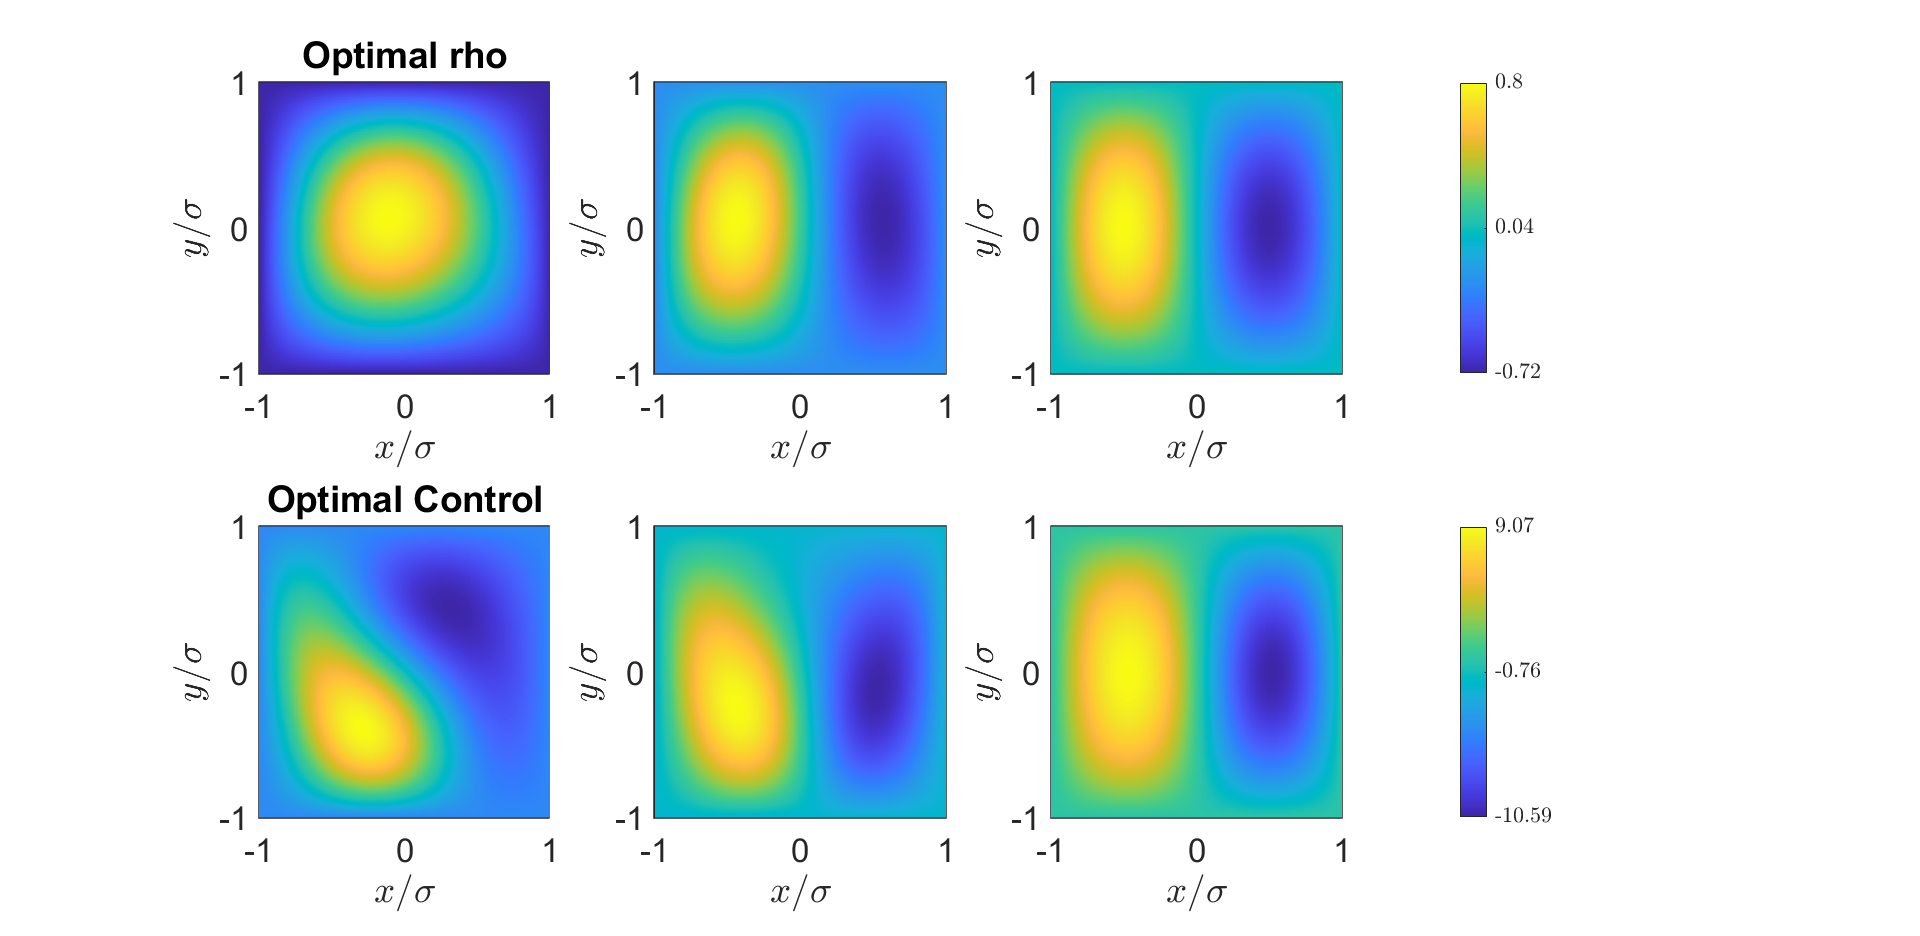
\includegraphics[scale=0.35]{SCEx2kn1V.png}
		\caption{Optimal $\rho$ and cost $w$, $\kappa = - 1$.} 
		\label{F2b}
	\end{figure}
	
	\section*{Flow Control Neumann}
	We choose 
	\begin{align*}
		\rho_0 &= 0.25\\
		V_{ext} &= ((x_1 + 0.3)^2 - 1)((x_1-0.4)^2 - 0.5)
		((x_2 + 0.3)^2 - 1)((x_2-0.4)^2 - 0.5)\\
		\hr &= (1-t)0.25 + t(1/1.3791)\exp{(-2((x_1+0.2)^2 + (x_2+0.2)^2))}
	\end{align*}
	We choose the domain $[-1,1]^2$ with a time horizon $(0,1)$. We have $N = 20$, $n = 11$. 
	For $\beta = 10^{-3}$, $\kappa = 1$ we get $J = 0.0059$, $J_1 = 0.0033$ and $J_2 = 8.4178$ (compare to $\beta = 10^3$ with $J = 0.0336$). For $\kappa = - 1$ we get $J = 0.0030$, $J_1 = 0.0019$ and $J_2 = 4.1185$ (compare to $\beta = 10^3$ with $J = 0.0214$).
		\begin{figure}[h]
		\centering
		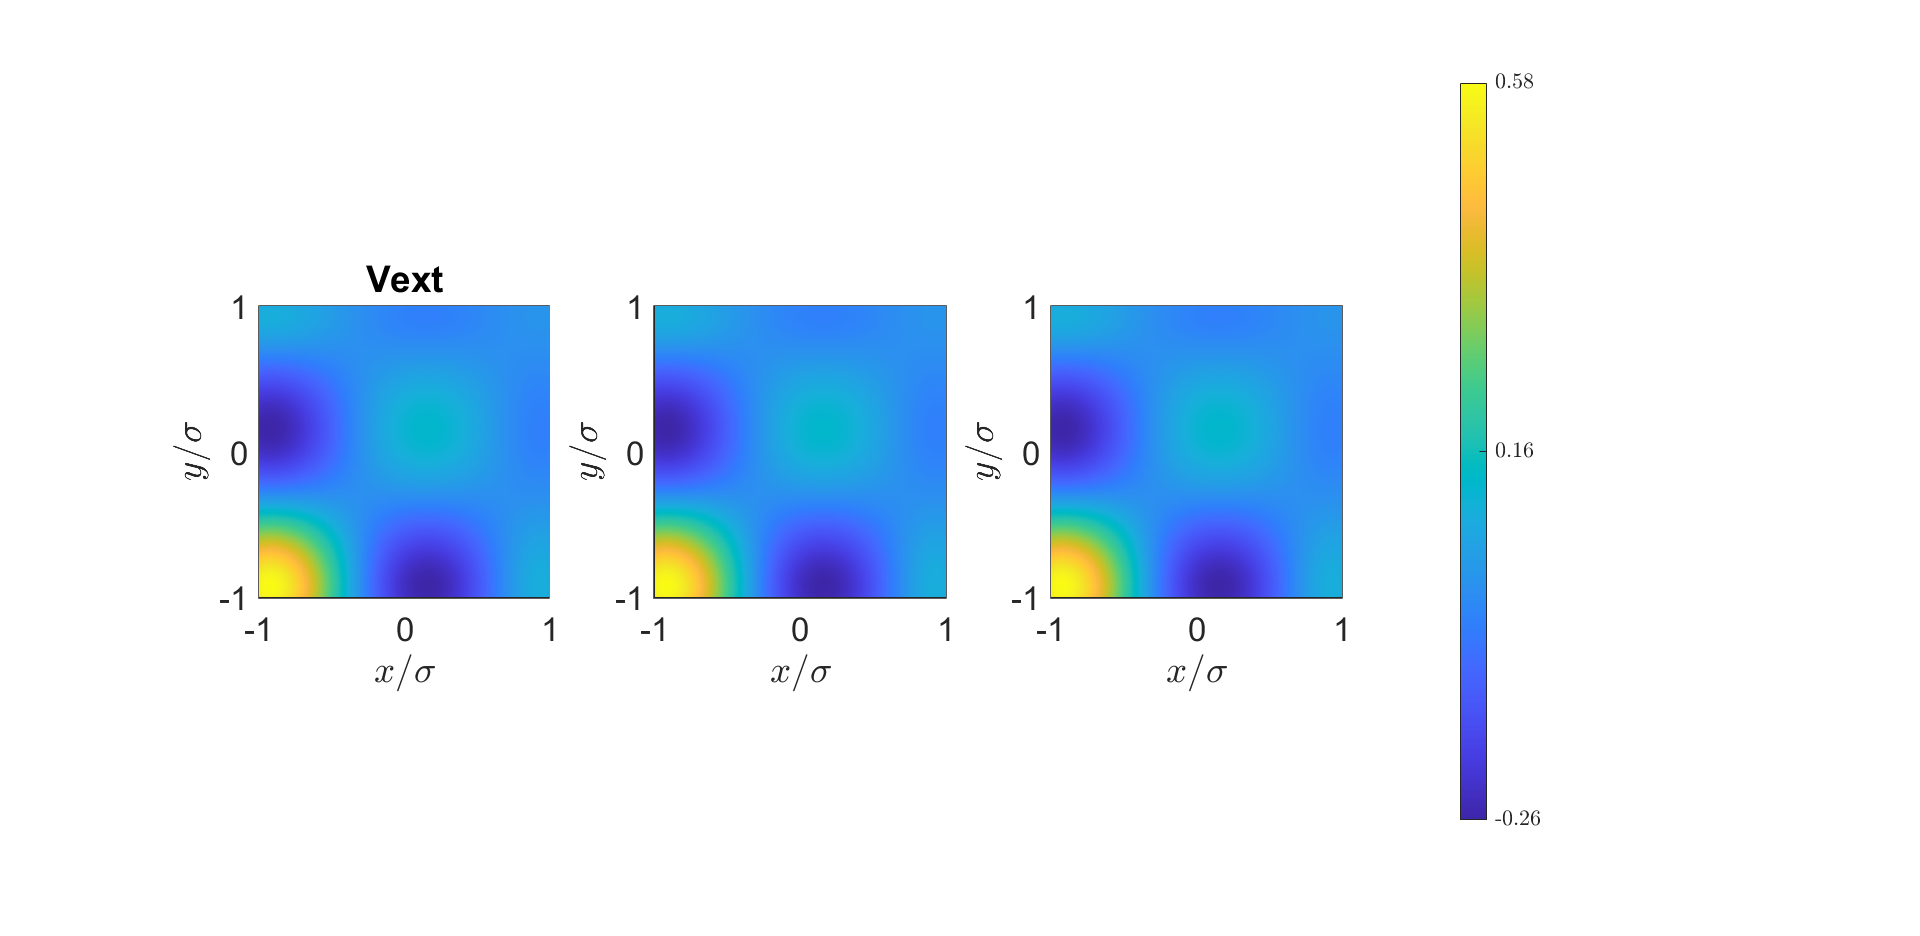
\includegraphics[scale=0.35]{VextEx4.png}
		\caption{$V_{ext}$ corresponding to results in Figure \ref{F3}.} 
		\label{F3a}
	\end{figure}
	\begin{figure}[h]
		\centering
		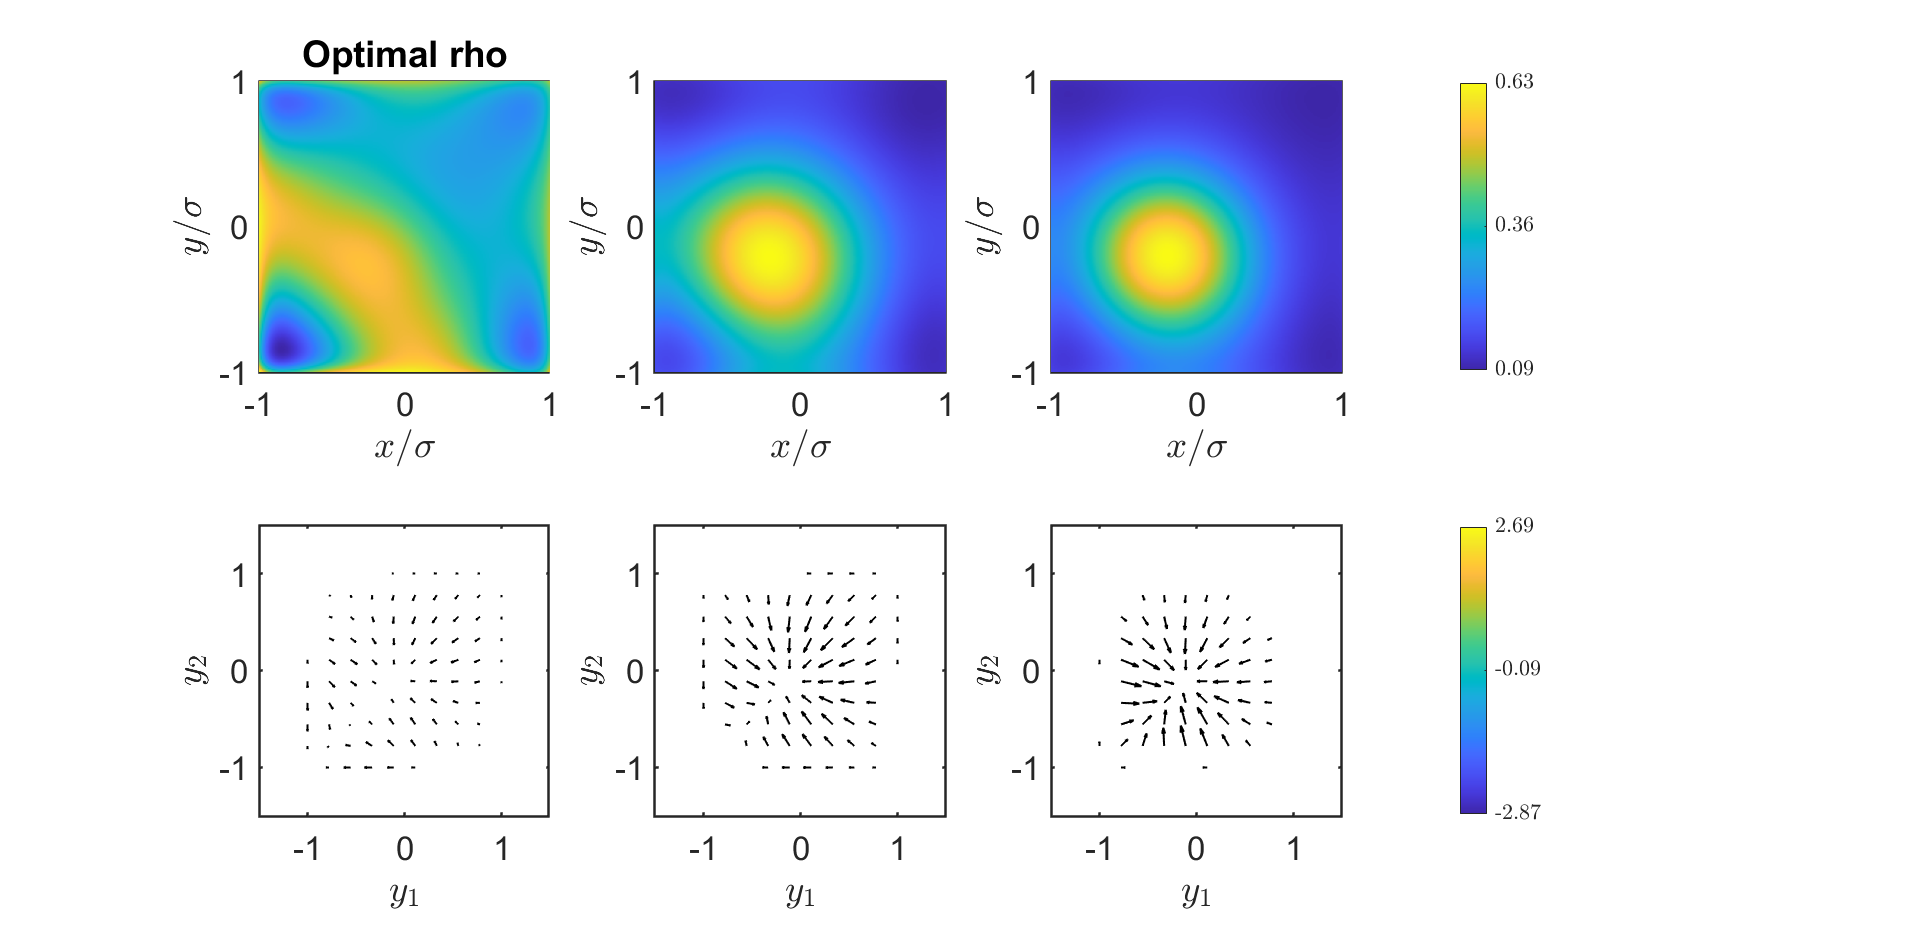
\includegraphics[scale=0.35]{FCEx2k1.png}
		\caption{Optimal $\rho$ and cost $w$, $\kappa = 1$.} 
		\label{F3}
	\end{figure}
	\begin{figure}[h]
		\centering
		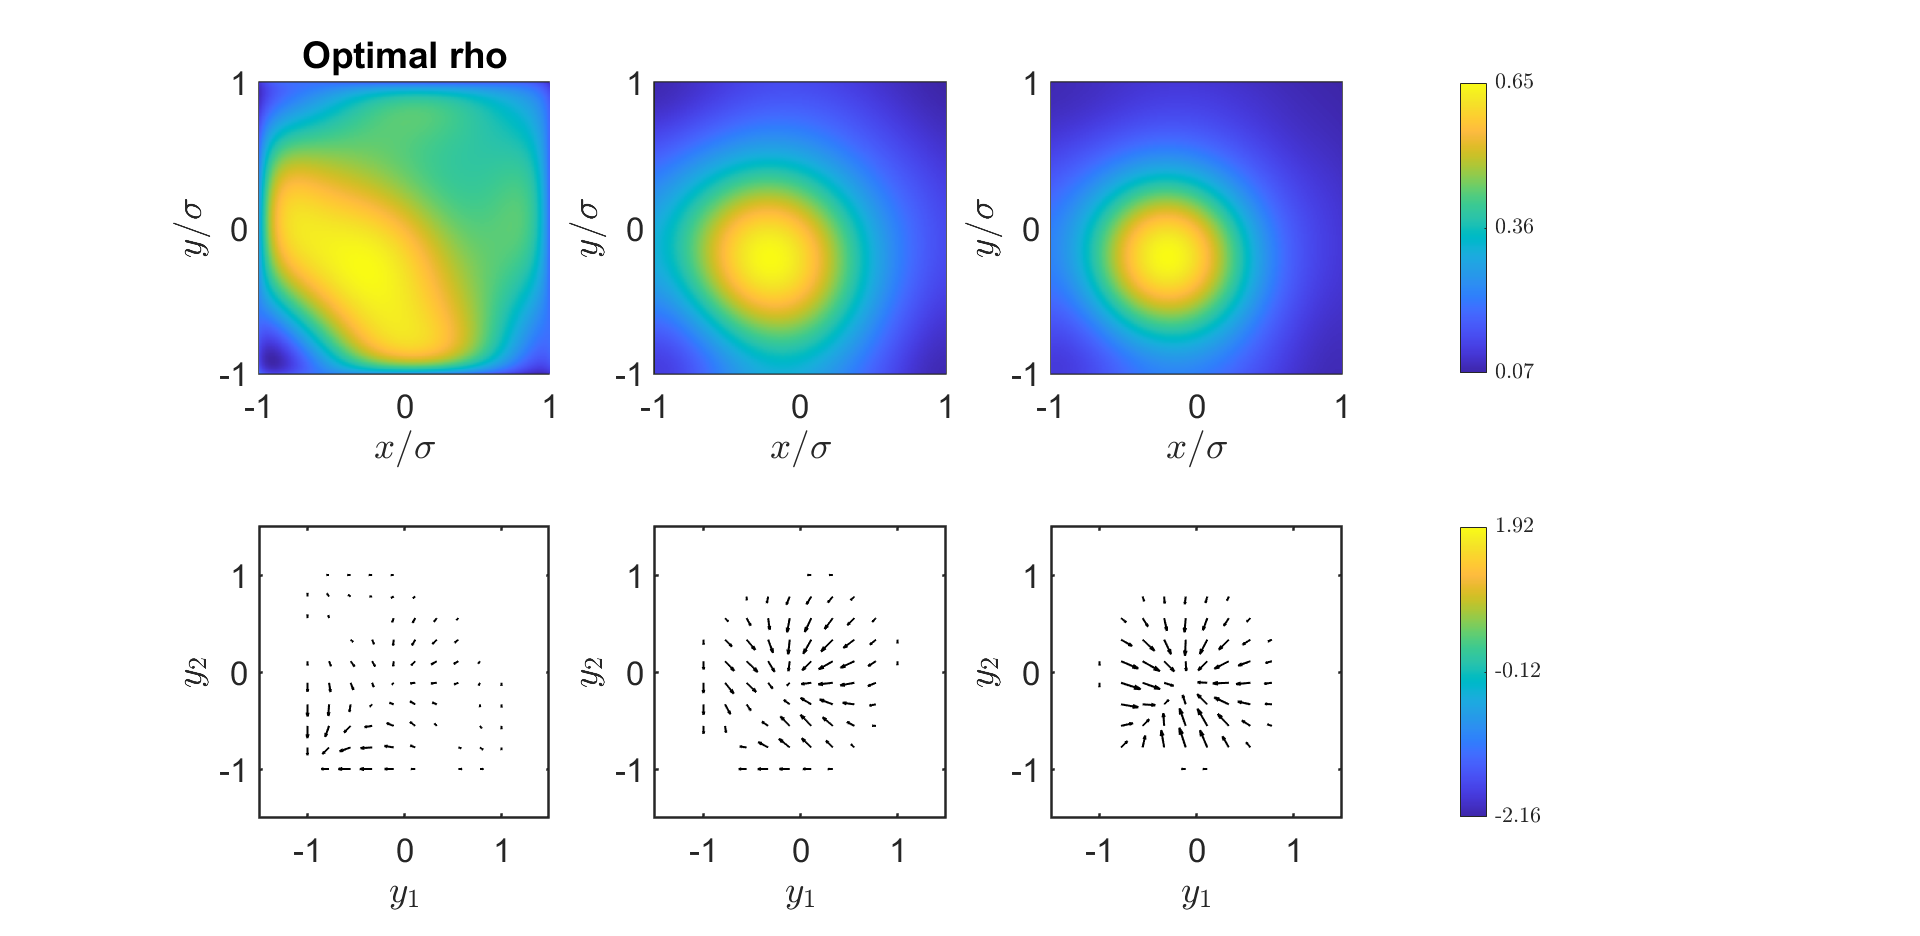
\includegraphics[scale=0.35]{FCEx2kn1.png}
		\caption{Optimal $\rho$ and cost $w$, $\kappa = - 1$.} 
		\label{F3b}
	\end{figure}
	\section*{Flow Control Dirichlet}
	
	For this example we need more points. In the following $N = 25$, but that's still not enough. 
	We choose 
	\begin{align*}
		\rho_0 &= (0.25\pi)^2\cos(\pi x_1/2)\cos(\pi x_2/2)\\
		\hr &= (1 - t)(0.25\pi)^2\cos(\pi x_1/2)\cos(\pi x_2/2) + t(0.5(0.25\pi)^2\sin(\pi x_1)\sin(\pi x_2/2 - \pi/2))
	\end{align*}
	\begin{figure}[h]
		\centering
		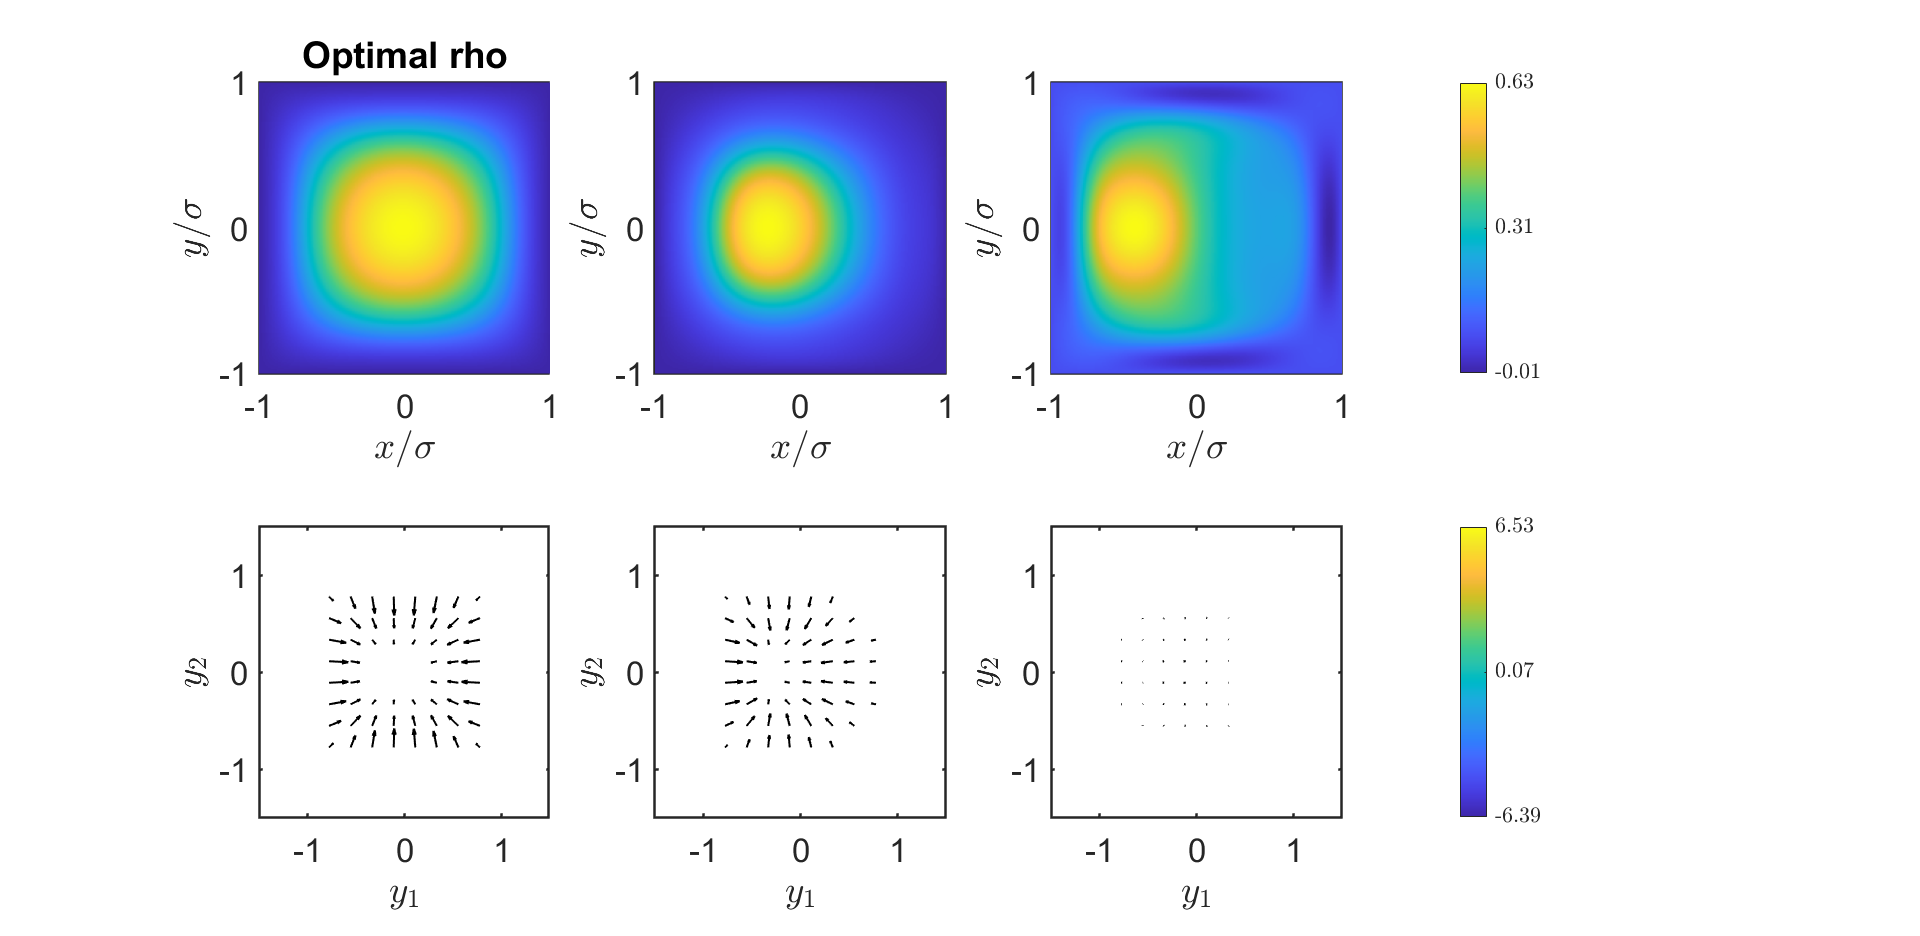
\includegraphics[scale=0.35]{FCEx1k1.png}
		\caption{Optimal $\rho$ and cost $w$, $\kappa = 1$.} 
		\label{F4}
	\end{figure}
	\begin{figure}[h]
		\centering
		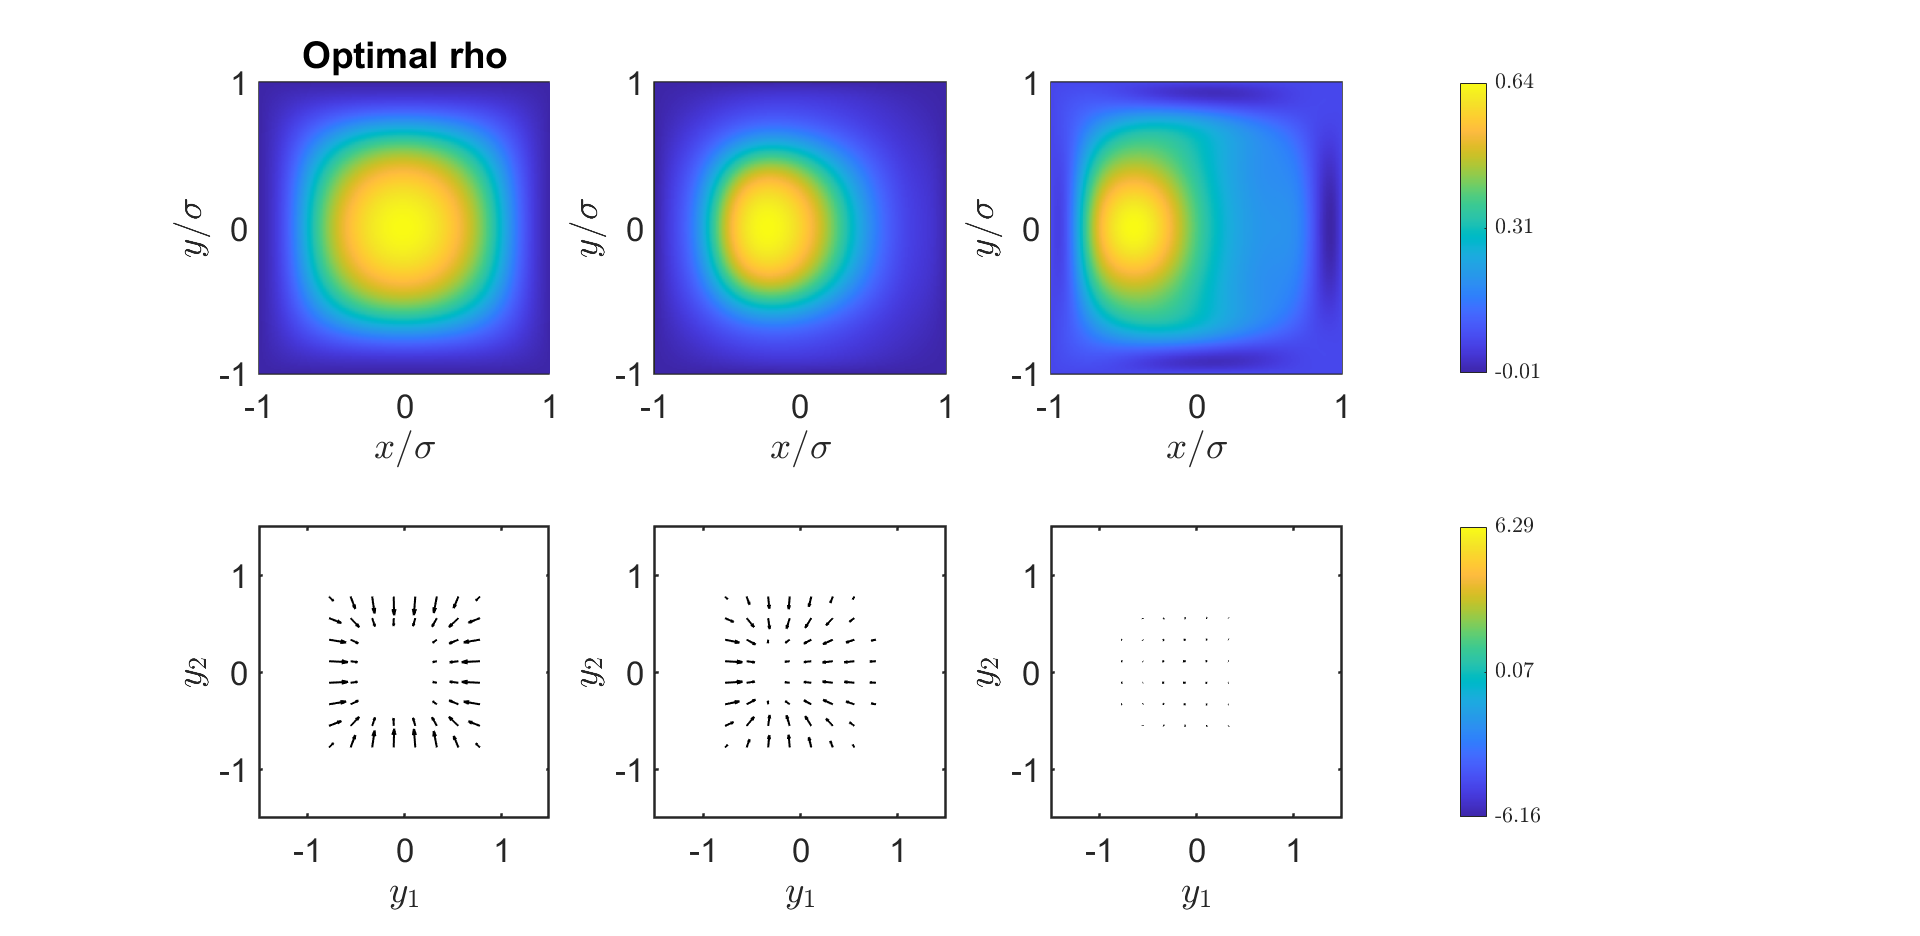
\includegraphics[scale=0.35]{FCEx1kn1.png}
		\caption{Optimal $\rho$ and cost $w$, $\kappa = - 1$.} 
		\label{F4a}
	\end{figure}
	
	\begin{figure}[h]
		\centering
		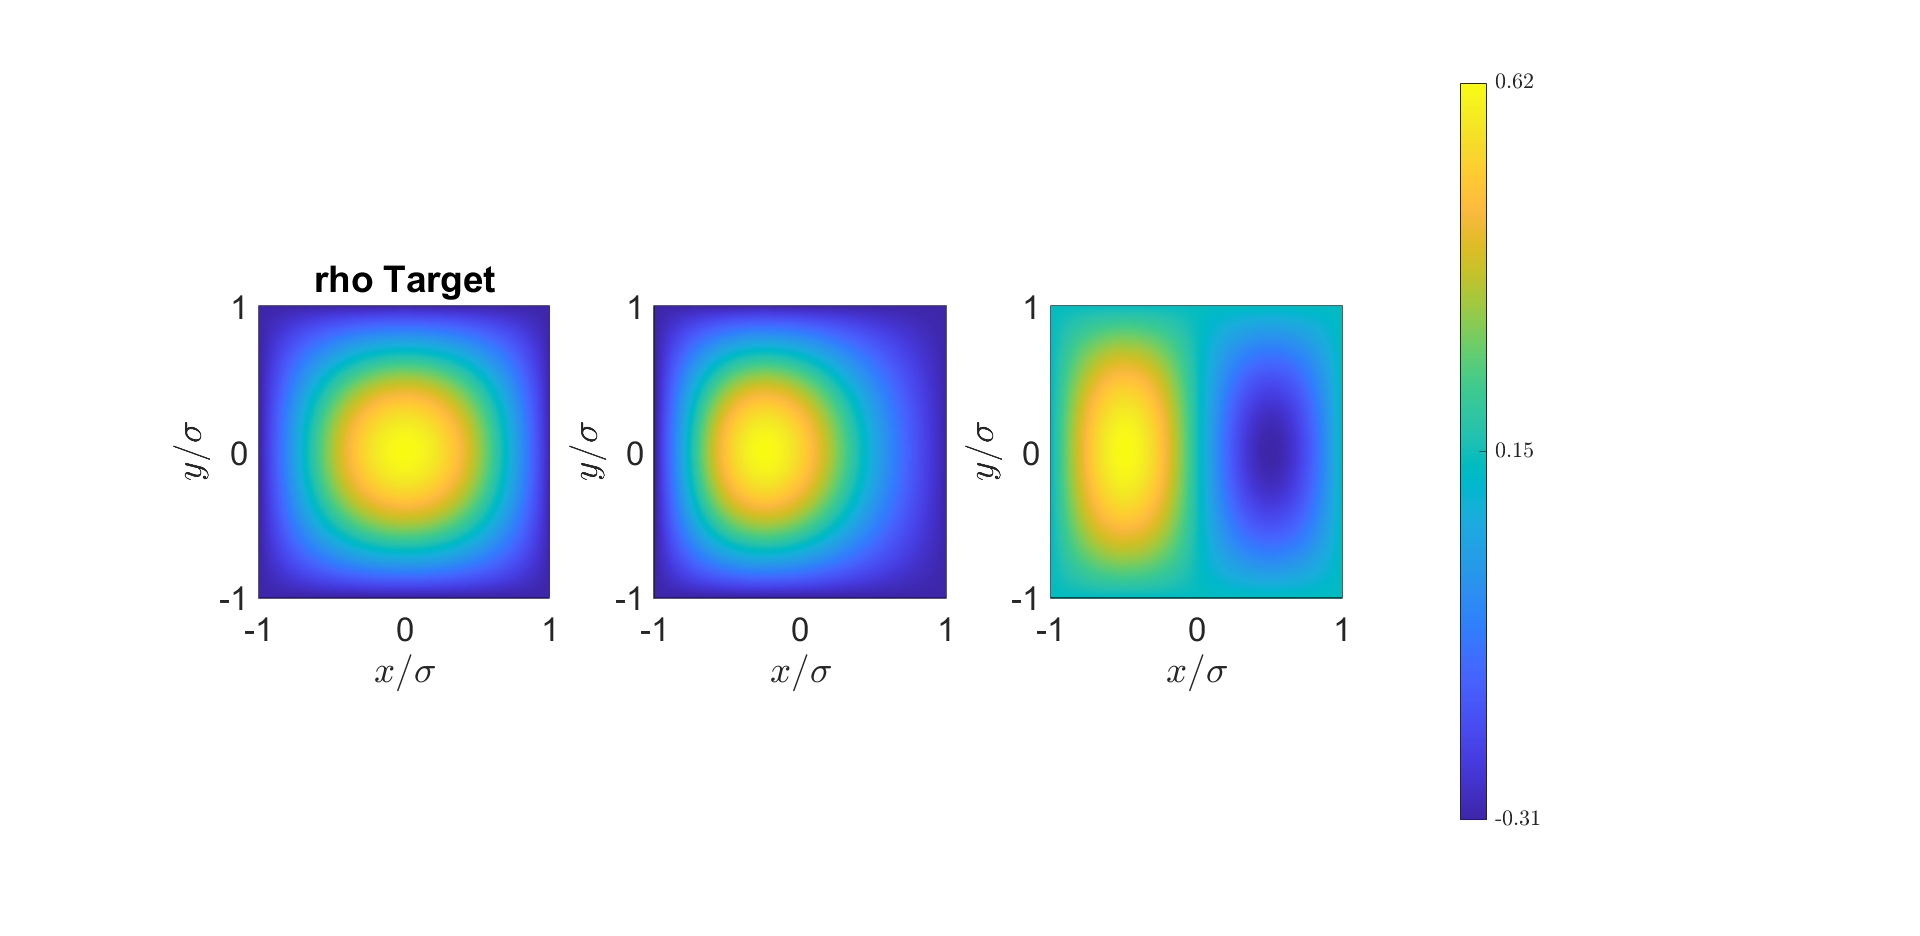
\includegraphics[scale=0.35]{FCEx1Target.png}
		\caption{Target $\rho$.} 
		\label{F4b}
	\end{figure}
	
	
	
\end{document}